% !TEX root = ../main.tex

\chapter{Introduction}
\label{ch:introduction}

\section{Reinforcement learning}
Reinforcement learning is a type of machine learning that focuses on training agents to make decisions in dynamic environments in order to maximize a reward signal. It is distinct from other paradigms such as supervised learning, which uses labeled data to predict outputs for unseen data, and unsupervised learning, which seeks to find patterns in unlabeled data. In addition to being a problem that can be addressed with specific solution methods, reinforcement learning is also the field of study that examines this problem and its potential solutions. Overall, the goal of reinforcement learning is to teach agents to make optimal decisions in order to achieve a desired outcome or reward.(\cite{sutton_reinforcement_2018}).

\vspace{5mm}

Classical reinforcement learning involves the interaction between two main components: an environment and an agent. The environment is represented by a current state that provides information about the "world" in which the agent is located, and the agent is the individual who performs actions within this environment. In each interaction, the agent receives observations based on the current state of the environment and selects an action to take. This action is then transmitted to the environment, which updates its internal state and provides feedback to the agent in the form of observations and a reward. The reward signal indicates whether the action was suitable for completing the task, while the observations provide an overview of the updated environment. Figure~\ref{fig:RL_main_loop} illustrates one timestep of interaction between the agent and the environment.
\begin{figure}[!ht]
\centering
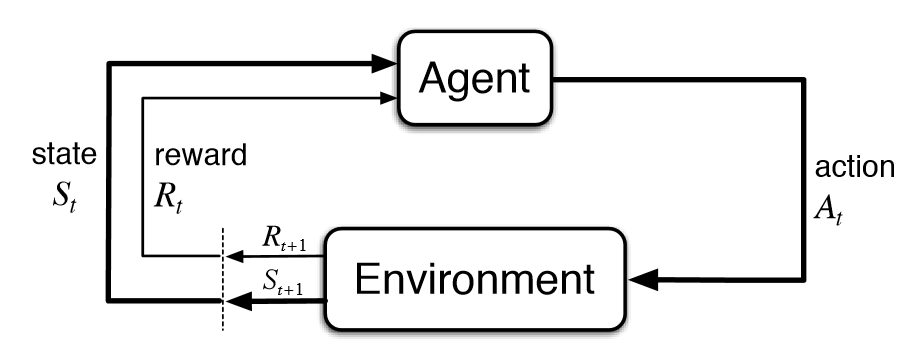
\includegraphics[width=.6\textwidth]{RL_main_loop}
\caption[Main interaction of the agent and the environment in reinforcement learning]{
  \textbf{Main interaction of the agent and the environment in reinforcement learning.}
  At the beginning (timestep $t$) the agent gets the observation $S_t$ and the reward $R_t$ from the environment. The agent performs then action $A_t$ and sends it to the environment. The environment changes its state and returns a new observation $S_{t+1}$ and a new reward $R_{t+1}$.
  
 }
\label{fig:RL_main_loop}
\end{figure}

\vspace{5mm}

In reinforcement learning, the policy is a key element of the framework that determines the actions an agent should take in different states of the environment. The policy is represented by a mapping from states to actions, and it can be either deterministic or stochastic. Deterministic policies specify a single action to take in each state, while stochastic policies specify probabilities for different actions to occur. The reward an agent receives depends on the chosen policy, and the sequence of states reached by the agent is called a Markov chain. This mathematical concept models systems that change over time in a way that depends only on the current state and not on the history of past states.(\cite{sutton_reinforcement_2018}).

The value function is a key concept in reinforcement learning that allows us to evaluate the effectiveness of different policies.$V_{\pi}(s)$ defines the expected total reward that an agent can expect to receive by following the policy $\pi$, starting from state $s$. One way to compute the value function is using the Bellman equation, which expresses the value of a state in terms of the values of its successors(\cite{barron_bellman_1989}). However, the Bellman equation does not have a closed-form solution, which makes it challenging to compute the value function in practice.
The value function can be used to define an optimal policy, which is the policy that is expected to maximize the reward over time. Another way to analyze policies is using the Q-function.$Q_{\pi}(s, a)$ is defined as the expected total reward acquired by the agent following policy $\pi$ starting from state $s$ and taking action $a$. The Q-function can be related to the value function through the equation $V_{\pi}(s) = Q_{\pi}(s, \pi(s))$. A common method for finding the optimal Q-function is Q-learning, which is an iterative process that updates the Q-function based on experience (\cite{watkins_q-learning_1992}). 

\vspace{5mm}

Reinforcement learning is well-suited for autonomous systems that learn to achieve a desired outcome through trial and error. However, this paradigm presents a unique challenge that is not encountered in supervised or unsupervised learning: balancing exploitation and exploration. Exploitation refers to the process of repeating actions that have resulted in positive rewards in the past, in order to maximize the cumulative reward. On the other hand, exploration involves trying new actions in order to potentially discover higher rewards and avoid getting stuck in a local optimum. Finding the right balance between these two approaches is crucial for the success of the learning process.

While reinforcement learning has been effective in solving a range of tasks, it has also encountered challenges in real-world applications (\cite{zhu_ingredients_2020}). In this thesis, however, the paradigm is sufficient for addressing the desired tasks. Overall, reinforcement learning offers a powerful tool for training agents to make decisions in dynamic environments and optimize for a given reward signal.

\section{Black-Box Optmization}

In mathematics, optimization refers to the process of finding the maximum or minimum value of an objective function. Neural networks, for example, try to find the best weights for approximating an underlying function using techniques such as backpropagation and gradient descent. However, these techniques require knowledge of the derivative of the function, which may not always be available or may be too complex to compute (\cite{schaul_studies_nodate}). Black-box optimization is a method that does not rely on any assumptions about the function or its properties, and can be used to optimize any function approximator. It is based on a feedback score similar to reinforcement learning, and the parameter set is improved based on this score (\cite{anderson_introduction_1995}).

Black-box optimization methods are generally less efficient than traditional techniques such as gradient descent because they do not take advantage of information about the structure of the function being optimized. This means they must explore a larger space of possible solutions, which can be time-consuming. However, black-box optimization methods can be effective in situations where the function being optimized is highly complex or has a large number of variables, and traditional methods may not be applicable. They are also flexible and can be applied to a wide range of problems without requiring any knowledge of the function being optimized

\subsection{Evolution strategies}

Evolution strategies (ES) is a class of evolutionary algorithms that is specialized for optimization of continuous variables. Inspired by natural evolution, ES is a black-box optimization algorithm that uses a process of mutation and selection to search for good solutions to a given problem. In the main loop of the algorithm, new individuals are created by mutating the parent individuals of the current generation. An individual in the context of ES refers to a specific set of parameters being optimized by the algorithm. A population is a group of individuals being considered by the algorithm at a given time, and a generation refers to one iteration of the main loop. The fitness of an individual is a measure of its performance or quality, based on the feedback score provided by the algorithm.

The main loop of the ES algorithm consists of creating new individuals from the parent individuals of the current generation, evaluating their fitness, and selecting the best-performing individuals to be the parent individuals for the next generation. This process continues until a sufficient solution is found, as determined by a stopping criterion. Algorithms differ in the number of offsprings created per generation, the number of selected individuals for the next generation, and how the mutation process is performed (\cite{salimans_evolution_2017}). Other than gradient-descent based methods, ES generates multiple individuals and by that explores different areas or paths of the optimization space independently, which can be beneficial for avoiding local optima and solving real-world problems that may require sophisticated exploration mechanisms.


\subsection{Covariance Matrix Adapation Evolution Strategy}

\section{Binary trees}

Trees are a commonly used data structure in mathematics and computer science that are composed of nodes and edges. A tree is an undirected, connected, acyclic graph, which means that it consists of a set of nodes that are connected by edges, but there are no loops or cycles in the graph. In a tree, a node that connects other nodes is called a parent node, and the nodes that are connected to it are called children nodes. The node at the top of the tree, which has no parent nodes, is called the root node, and the nodes at the bottom of the tree, which have no children, are called leaf nodes. The levels of a tree are determined by the distance from the root node, with the root node being at level 0 and the nodes connected to it being at level 1, and so on. Nodes on the same level are called sibling nodes.

Binary trees are a special type of tree in which all nodes except for the leaf nodes have at most two children nodes. These children nodes are typically referred to as the left node and the right node, respectively. An example of a binary tree is shown in Figure \ref{fig:binary_tree}.

\begin{figure}[!ht]
\centering
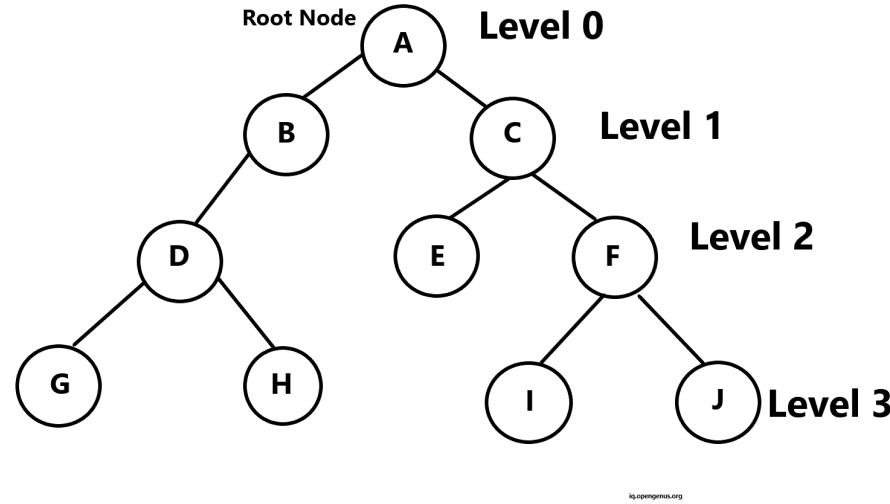
\includegraphics[width=.6\textwidth]{binary_tree}
\caption[Binary tree with letters representing the data]{
  \textbf{Binary tree with letters representing the data}
  }
\label{fig:binary_tree}
\end{figure}

\section{Open AI Gym}





